% !TEX root = ../thesis.tex
%
\chapter{Related Work}
\label{sec:related}

As Runtime Monitoring and Verification is a widely researched field, multiple approaches have been developed and new approaches are presented all the time.

As stated in~\cite{Havelund2008} most approaches are geared towards software written in Java, while many critical systems are written in C.
Additionally there are countless other systems that could benefit from monitoring and verification written in other programming languages.
\Gls{tessla} is a specification language over streams, which has no assumptions on the environment of the system that produces the streams.
Using \gls{tessla}  as the base for our monitoring approach, we recognized the possibility to decouple the monitoring platform from the monitored program.
This means that the runtime developed for \gls{tessla} is not restricted to monitor programs written in a specific language but can monitor anything that can produce streams of data.

To show that the runtime is valuable in the context of existing approaches we will look at ways to generate traces from systems during their execution.
Based on the generated traces we benchmarked out runtime to evaluate how it scales with respect to different characteristics of specifications and the plattform it is run on.

The following chapter will summarize the approaches that are available in the field of \gls{rv} and how they influenced \gls{tessla} and the runtime we implemented.

\section{\glsentryname{rv} Techniques for C Programs}
\label{sec:related:c_programs}

Most \gls{rv} approaches are developed for Java and the \gls{jvm} and therefore they are not usable for a large class of software not written in Java.
In particular C and \CC are used in a wide variety of safety critical systems, including aircrafts and energy plants.
While \gls{tessla} as a language and the implemented runtime is independent of the platform of the monitored program, the domain of C programs and especially embedded software has a special focus in this thesis.
Therefore in this section we will look at some existing approaches to monitor C programs and in Section~\ref{sec:related:traces} we will discuss ways to generate trace data from such programs.

\subsection{Copilot}
\label{sec:related:c_programs:copilot}

The realtime runtime monitor system Copilot was introduced in~\cite{Pike2010}.
Copilot is designed to overcome the shortcomings of existing \gls{rv} tools in regards to hard-realtime software written in C.

To accomplish this goal Copilot defines characteristics that a monitoring approach has to fullfill to be considered valuable for this domain.
The four principles are:

\begin{description}
  \item[Functionality] Monitors cannot change the functionality of the observed program unless a failure is observed.
  \item[Schedulability] Monitors cannot alter the schedule of the observed program.
  \item[Certifiability] Monitors must minimize the difficulty in re-validating the observed program. In particular, monitoring must be accomplished without modifying the observed programs source code.
  \item[SWaP overhead] Monitors must minimize the additional overhead required including size, weight, and power (SWaP).
\end{description}

The monitors follow a sampling based approach, where at specified steps the values of global variables are observed and the monitors are evaluated on the observed values.
While sampling based approaches are widely disregarded in \gls{rv} because they can lead to both false positives and false negatives, \cite{Pike2010} argues:

\begin{quote}
  In a hard real-time context, sampling is a suitable strategy.
  Under the assumption that the monitor and the observed program share a global clock and a static periodic schedule, while false positives are possible, false negatives are not.
\end{quote}

A special detail of Copilot is that monitors are not inlined into the program but can be scheduled as independet processes.
The implementation of the \gls{tessla} runtime in this thesis follows a similar approach.
Our runtime is a totally independent program and therefore also enjoys some of the gains with respect to the specified four characteristics.
Because the runtime works with all kinds of traces, it is insignificant how these traces are produced.
Our runtime can work with traces based on sampling, working in a similar fashion as Copilot, or by actually instrumenting code to generate traces, which might alter the semantics of the monitored program.

\subsection{\glsentryname{rmor}}
\label{sec:related:c_programs:rmor}

\gls{rmor}~\citep{Havelund2008} is another approach for monitoring C programs.
\gls{rmor} transforms C code into an \emph{armored} version, which includes monitors to check conformance to a specification.

Specifications are given as a textual representation of state machines which is strongly influenced by \gls{rcat}~\citep{Smith2008}.
The specifications are then interweaved into the program using \gls{cil}~\cite{Necula2002}.

The specifications considered in \gls{rmor} work on the level of function calls and state properties like \emph{write may never be called before open was called}.
Because software developers are often working at the same abstraction level (in contrast to assembler or machine instructions), they can define specifications without having to learn new concepts.
The \gls{tessla} runtime supports the definition of traces at the same abstraction level (function calls, variable reads and writes).
This is used in most of the tests in \Cref{sec:evaluation:runtime_examples}.

Because \gls{rmor} specifications are interweaved into the program, their observations can not only be reported but also used to recover the program or even to prevent errors by calling specified functions when a critical condition is encountered.
The \gls{tessla} runtime does not support this functionality out of the box as its primary purpose is testing and offline monitoring.
In \Cref{sec:conclusion:further_work:error_prevention} we will look at possible extensions to enable communication from the monitor back to the monitored program.

\section{Distributed Verification Techniques}
\label{sec:related:distributed}

Many works in the field of \gls{rv} do not consider parallelism and distributed systems.
There are two aspects to this challenge: monitoring programs that are run in a distributed fashion on the one hand, and using parallelism and distribution to implement monitors on the other.

Monitoring distributed programs carries an inherent problem: events are no longer globally ordered.
This led to algorithms like Lamport timestamps~\citep{Lamport1978} and vector clocks~\citep{Fidge1988}.
The distribution of the monitored system, and therefore of the events, must be expressable in the language that is used to write specifications about the system.
Two examples for such a specification language are presented in \cite{Sen2004} and \cite{Ehrich2000}.
\cite{Mostafa2015} presents a way to monitor distributed programs that uses \gls{ltl} as the specification language, but requires the presence of a global state which is cosntructed using Lamport timestamps.
\cite{Mostafa2015} presents a method to implement distributed monitors that have to communicate with one another.

While the \gls{tessla} specification language does not include mechanisms to explicitly reason about distributed properties, the \gls{tessla} runtime does not care about the environment of the monitored program, so it does not distinguish between traces from distributed and non distributed programs.
As we will see in \Cref{sec:implementation:tesslaserver} this means that \gls{tessla} can be adopted to monitor at least some characteristics of a distributed system.
But more importantly, the runtime takes parallelism and distribution as one of its core concepts as we will explain in the next chapters.

The other challenge of parallelism and distribution is how these features can be used to implement monitoring algorithms.
Since modern systems often contain many processors or cores it is important to study how to exploit parallelism when building monitors, especially when performance of the monitor is important.

The work in~\cite{Attard2016} uses the Erlang plattform to implement a highly distributed monitoring algorithm for a branching time logic called \gls{mhml}.
The approach works by synthesizing formulas into \emph{submonitors} which can then be run in parallel.
The verdicts from these monitors are combined to form a global verdict.
For example the formula \(\Phi \vee \Psi\) can be synthesized as two \emph{submonitors}, one for \(\Psi\) and one for \(\Phi\).

The \gls{tessla} runtime follows a similiar approach where each part of the specification is implemented as an independent actor.
These actors can then be scheduled by the environment in a parallel fashion.
In \Cref{sec:implementation:tesslaserver} we will look at this architecture more closely.

\section{Stream Based Specification Techniques}
\label{sec:related:stream_based}

Specifications in the field of \gls{rv} are defined over finite words, meaning a finite sequence of events.
But some works take another perspective on the problem and look at the sequence of properties as streams of data.
As \gls{tessla} takes this approach we will look at other work that promoted this view and how it can be used to incorporate techniques from other fields into \gls{rv}.

\subsection{\glsentryname{lola}}
\label{sec:related:stream_based:lola}

The concepts of \gls{lola}~\cite{DAngelo2005} are very similar to the ones of \gls{tessla}.
The biggest difference between these two approaches is that streams in \gls{lola} are based on a discrete model of time while \gls{tessla} uses a continuous timing model highlighted in \Cref{sec:related:tessla}.

The specification language of \gls{lola} is very small (expressions are built upon three operators) but the expressiveness surpasses \acrlongpl{tl} and many other formalisms for finite traces \citep{DAngelo2005}.
Expressions in \gls{lola} are built by defining streams from other streams.
Therefore streams depend on other streams and they can be arranged in a weighted dependency graph, where the weight describes the amount of steps a generated stream is delayed compared to the stream in its definition.
In contrast to \gls{tessla} streams in \gls{lola} can depend on themself and therefore the dependency graph can contain cycles.
Based on this graph a notion of efficiently monitorable properties is given in \citep{DAngelo2005} which also presents a monitoring algorithm.

\Cref{listing:lola_spec} shows a small specification written in \gls{lola}.
This example shows the usage of integer streams, which allows \gls{lola} the use of counters and therefore enables it to express context-free properties.

\begin{lstlisting}[escapeinside=``,numbers=none,float,label=listing:lola_spec, caption={[A specification written in \gls{lola}]A \gls{lola} specification describing the property that the number of \emph{a}\'s in a stream shall never be less then the number of \emph{b}\'s}]
s = s[-1, 0] + ite((a `\(\wedge\ \neg \)`b), 1, 0) + ite((b `\(\wedge\ \neg \)`a), −1, 0)
trigger(s `\(\leq\)` 0)
\end{lstlisting}

\Gls{lola} was recently extended in~\cite{Faymonville2016} with two new features:  template stream expressions, which allow input data to be carried along the stream, and dynamic stream generation, where new monitors can be invoked during the monitoring process for the monitoring of new subtasks on their own time scale.
These extensions add the concept of \emph{slicing} with template streams, which enables the generation of  parameterized streams.
A parameterized stream, also called template stream, is a mechanism to generate dynamically concrete streams from one template stream by \emph{slicing} it with respect to some data.
For example, a template stream could be used to monitor logins of individual users, where one \emph{slice} is generated for each user.
Adding parameterization to \gls{tessla} was discussed but is not currently implemented yet.

\gls{tessla} takes concepts of \gls{lola} and applies them to a continuous model of time and introduces a language and a rich set of functions that can be applied to streams.
The dependency graph is a core concept of \gls{tessla} and is used to check if specifications are valid and is also the core concept to evaluate specifications over traces in this thesis.

\subsection{BeepBeep 3}
\label{sec:related:stream_based:beepbeep}

The project BeepBeep aims to introduce concepts from the field of \gls{cep} to \gls{rv}.
The third version of BeepBeep is presented in~\cite{Hall2011} where different concepts from \gls{cep} are applied to problems of \gls{rv}.
BeepBeep implements a system for evaluating specifications over synchronous event streams.
It exposes two ways to express specifications: an \gls{api} in Java and the language \gls{esql}.

The evaluation model of BeepBeep is very similiar to the one implemented for \gls{tessla} in this thesis: events enter the system through sources, flow through multiple processors which perform transformations and in turn can lead to the generation of an output.
The central unit of computation are called processors: processors transform multiple input streams into multiple output streams.
A processor can only perform a transformation when there is at least one event buffered at each input stream.
The combination of the first event on each buffer is called the \emph{front}.
Whenever a front can be formed the processor is invoked to perform its work and generate new outputs based on the front
We will reuse this terminology in \Cref{sec:implementation:tesslaserver} when we talk about the way computations in \gls{tessla} work.

\section{\glsentryname{tessla}}
\label{sec:related:tessla}

The implemented runtime and the theoretic work of this thesis is built upon the \gls{tessla} project from~\cite{Decker2016}, that defines a syntax and a formal semantic of the \gls{tessla} specification language.

Specifications in \gls{tessla} are based on streams of data.
Streams are the representation of data over time, for example the value of a variable in a program or the temperature of a processor.
To model streams \gls{tessla} defines a timing model.
That model is based on timestamps that are isomorphic to real numbers \(\mathbb{R}\).
\Cref{fig:chap2:sec_tessla:streams} illustrates how streams behave over time.

\begin{figure}
  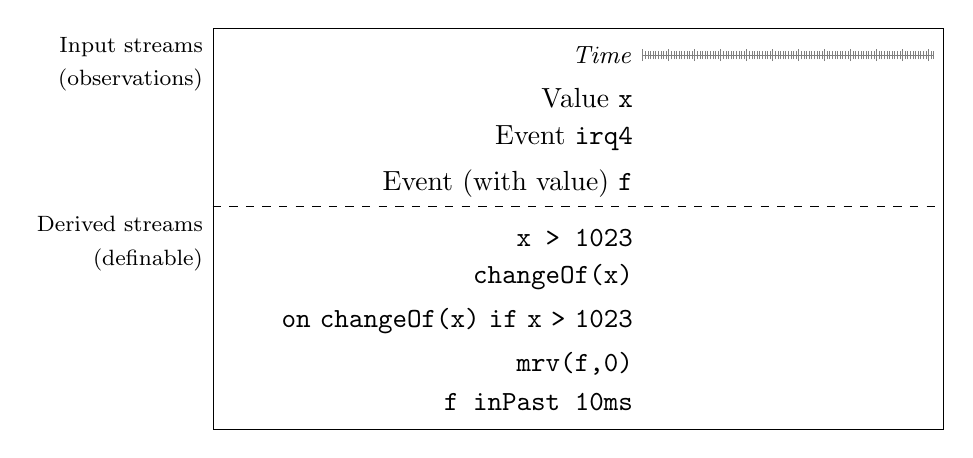
\begin{tikzpicture}

\matrix[column sep = 0.5em, draw] (m) {
  \node[anchor = east] {\small \textit{\textrm{Time}}}; \& \draw[help lines] (0,-0.05) grid[xstep=0.033] (3.7,0.05);
     \draw[gray] (0,-0.075) grid[xstep=0.33] (3.7,0.075); \\[0.5ex]
  \node[anchor = east] (m-1-2) {Value \texttt{x}}; \& \timing[name=m-2-2] at (0,-0.15) {2D{998}N(x1)2D{42}3D{2012}3D{1280}DD{10}DD{1404}};\\
%
  \node[anchor = east] (m-1-3) {Event \texttt{irq4}};
    \& \timing[name=m-2-3] at (0,-0.15) {ZZZ \n{} Z \n{} ZZZZ \n{} ZZ \n{} ZZZ \n{} Z}; \\
%
  \node[anchor = east] (end-inputs) {Event (with value) \texttt{f}};
    \& \timing[name = end-inputs-2] at (0,-0.15) {Z \n{17} ZZZZZZZ \n{98} Z \n{0} ZZZZ \n{23} Z}; \\[0.5em]
%
     \node[anchor = east] (m-1-5) {\texttt{x > 1023}};
  \& \timing[name=m-2-5] at (0,-0.15) {4L 6H 2L 2H}; \\
%
     \node[anchor = east] (m-1-6) {\texttt{changeOf(x)}};
  \& \timing[name=m-2-6] at (0,-0.15) {2Z \n{} 2Z \n{} 3Z \n{} 3Z \n{} 2Z \n{} 2Z}; \\
%
     \node[anchor = east, text width = 14.5em, align = right] (m-1-7) {
          \texttt{\textbf{on} changeOf(x) \textbf{if} x > 1023}};
  \& \timing[name=m-2-7] at (0,-0.15) {4Z \n{} 3Z \n{} 3Z 2Z \n{} 2Z}; \\
%
     \node[anchor = east] (m-1-8) {\texttt{mrv(f,0)}};
  \& \timing[name=m-2-8] at (0,-0.15) {D{0} 7D{17} D{98} 4D{0} D{23}}; \\
%
     \node[anchor = east] (m-1-9) {\texttt{f inPast 10ms}};
  \& \timing[name=m-2-9] at (0,-0.15) {L 2H 5L 3H 2L H}; \\
%
 };

\path[draw, dashed] (m.west|-end-inputs.south) edge (m.east|-end-inputs.south);

\path (m.north west) node[anchor = north east, align = right]
{\footnotesize{Input streams} \\ \footnotesize{(observations)}};

\path (m.west|-end-inputs.south) node[anchor = north east, align = right] {
  \footnotesize{Derived streams} \\ \footnotesize{(definable)}};

\end{tikzpicture}

  \caption{Visualization of \gls{tessla} stream model, taken from~\cite{Decker2016}}
\label{fig:chap2:sec_tessla:streams}
\end{figure}

The syntax of \gls{tessla} is concise, but can be used to define complex functions and specifications:

\begin{align*}
  spec\ \text{::= } &\textttbf{define } name[\textttbf{:}\ stype]\ \textttbf{:= } texpr |\\
                    & \textttbf{out } texpr |
                    spec\ spec\\
  texpr\ \text{:= } & expr[\textttbf{:}\ type] \\
  expr\ \text{:= }  & name \mid literal \mid name\textttbf{(}texpr(\textttbf{, }texpr)^*\textttbf{)}\\
  type\ \text{:= } & btype \mid stype \\
  stype\ \text{:= } & \textttbf{Signal<}btype\textttbf{>} \mid \textttbf{Events<}btype\textttbf{>}
\end{align*}

One of the main contributions of \gls{tessla} is the syntax which mimics modern programming languages and diverges from more clasical approaches in \gls{rv} that use more formal specification languages typically based on logics or automata.
This is an important step to enable practitioners without a strong theoretical background to adopt \gls{rv} techniques in their workflow.
While \gls{rv} has a lot of mechanisms to express specifications they often lack the ability to be intuitively understood.

There are many specification languages like \gls{ltl}~\citep{Pnueli77}, \gls{rltl}~\citep{Leucker2007}, \gls{ctl}~\citep{Clarke82} and many others that are geared heavily toward scientific work and theoretic reasoning.
When introducing new concepts, like realtime, this trend keeps up and formalism like \gls{tltl} from~\cite{Raskin1997}, \gls{stl} from~\cite{Maler2004} and \gls{mtl} from~\cite{Koymans1990} provide theoretical foundations to reason about realtime properties but formulas using these logics are even harder to understand than their non realtime counterparts.

One approach to make \gls{rv} more usage friendly is \gls{salt} presented in~\cite{Bauer2006} which acts as a frontend language to the more formal specification languages and can be translated into them.
\Gls{salt} unifies many different mechanisms, like specification patterns, nested scopes, exceptions, regular expressions and realtime.
\Cref{listing:salt_example} shows an example specification in \gls{salt} taken and adapted from~\cite{Dwyer1999} which specifies that on all three floors in a building, calling the elevator at floor \(\mathit{i}\) implies that it may pass at most two times at that floor without opening its doors, and that it must finally open its doors at that floor within 60 seconds.

\begin{lstlisting}[float,breaklines=true,label=listing:salt_example,caption={[Example \gls{salt} specification with realtime operators]An example specification in the \gls{salt} language taken from \cite{Bauer2006} defining behaviour of an elevator.}]
define max_twice_at_floor_before_open(i) := always (occurring[<=2] atfloor_$i$ between inclusive optional call_$i$ , exclusive optional open_$i$)
define max_60s_before_open(i) := always (call_$i$ implies eventually timed[<=60.0] open_$i$)
assert allof enumerate[1..3] as floor in max_twice_at_floor_before_open(floor) and max_60s_before_open(floor)
\end{lstlisting}

This specification shows, how \gls{salt} specifications are more intuitively understandable than logic formulas, for example by allowing to split the formula in multiple parts and assign meaningful identifiers to subformulas.

\Gls{tessla} and the runtime implemented in this thesis aim to combine many of the aspects that were presented in this Chapter: An understandable specification language like \gls{salt} that is able to express realtime properties, using streams of data as a central element like \gls{lola}, incorporate techniques from \gls{cep} like BeepBeep, and distribute the montitoring to many processors using Erlang and the actor model as shown in \cite{Attard2016}.

\section{Trace Data}
\label{sec:related:traces}

As in \gls{rv} we talk about monitoring of properties over traces, another important aspect is how traces can be extracted from a running program.
Many \gls{rv} tools solve this problem by using a technique called \emph{interweaving}: The code of the monitored program is changed in a way that the monitor becomes part of it, therefore the monitor becomes part of the program and has explicit access to the state of the running system.
Examples for this approach are AspectJ~\cite{Kiczales2001} and DiSL~\cite{Marek2012} for Java, and \gls{rmor}~\cite{Havelund2008} and \gls{rithm}~\cite{Navabpour2013} for C.
This approach is not feasible for the goals of the \gls{tessla} runtime, because we seek the portabilty that enables users to monitor multiple kinds of systems.

Therefore we are looking for ways to manipulate programs in a general way to emit trace data.

As a first step we seeked other projects to extract traces of data that can be used to evaluate the implemented runtime.
While there are many benchmarks available to test monitoring tools we were not able to find any that satisfied all of the characteristics that are needed for an evaluation of \gls{tessla}.
The next sections lists some of the benchmarks and evaluation tools that were surveyed and concludes with a tool that enabled the generation of suitable trace data.

\subsection{General Benchmarks for \glsentryname{rv} Tools}

The field of \gls{rv} lacks a common specification language and can be expanded to a wide variety of different properties to verify.
Therefore it is no surprise that there is no common benchmark that is applicable to all tools.
Nonetheless some benchmarks are occasionally used to compare the expressiveness of a new \gls{rv} tool.

The DaCapo benchmark~\citep{Blackburn2006} was introduced as a general purpose benchmark for the Java language.
It turned out that it can be used to benchmark monitor implementations and trace collection tools~\citep{Wu2016,Chen2007,Marek2012}.
Since Java was not the target architecture of our runtime the DeCapo benchmark was not used for the evaluation in this thesis.

The works in~\cite{Dwyer1999} can be seen as a benchmark for the expressiveness of a specification language.
It categorizes commonly monitored porperties into so called patterns like \emph{precedence}, \emph{absence} and \emph{response}.
While it would be valuable to test \gls{tessla} and the implemented runtimes against these patterns this would be a two step process.
First each pattern would have to be checked, if and how it could be expressed as a \gls{tessla} specification.
As a second step, if the pattern can be expressed, test trace data would have to be generated and only then the runtime could be evaluated using that pattern.
Since this thesis does not work on the \gls{tessla} language definition but only on the runtime we decided not to pursue this gial.

Another interesting project for evaluation of offline monitoring tools is TraceBench presented in~\cite{Zhou2014}.
TraceBench is a big set of traces collected from a distributed system running \gls{hdfs}.
During the collection errors of different categories were deliberately introduced, like network timeouts or data corruption.
The generated traces are organized in a hierarchy: if an event is produced as the effect of another event, for example a function call that leads to another function call, the second event is a child of the first.
Furthermore the traces contain the beginning and end of each event as a timestamp, making the traces suitable for \gls{tessla}.
Unfortunately it seems that the generated trace data has a problem: since events are produced in a distributed system the timestamps are faulty, for example some events started before their parent event.
Furthermore \gls{tessla} doesn't have a mechanism to express nested events as of now, meaning the traces would need to be manipulated before they could be used.

As a final benchmark we evaluated the \gls{crv}~\citep{Reger2016}.
\Gls{crv} has collected a set of benchmarks especially developed for the usage in monitoring algorithms.
It consists of three tracks: Java, C and offline.
While the C and offline track would have been very interesting the benchmarks don't contain any realtime properties.
Since the realtime fragment is an important part of \gls{tessla} we decided that the benchmark wasn't appropriate either.

\subsection{Tools to Generate Traces}

Since no suitable benchmark could be found the next step was to search for a tool that can be used to generate apropriate traces from programs during execution.
These tools can be categorized into static and dynamic instrumentation tools: static tools transform the source code of a program during compilation to include logging statements, dynamic ones only work at runtime and are not involved in the compilation process.

% DTrace PID
\subsection{CIL}

\Gls{cil} \cite{Necula2002} is a tool to write source-to-source transformations for C programs, therefore it is a static instrumentation tool.
\Gls{cil} implements ``a highly-structured clean subset of C'' in the OCaml language.
\Gls{cil} transforms a C program into an intermediate representation in OCaml.
\Gls{cil} will then apply transformations that are supplied by the programmer to the intermediate representation.
When all transformations are applied the program is written back as a normal C program.

Since \gls{cil} is able to represent the complete C90 standard and also extensions that are commonly used like the ones from GNU C, this tool can be used to write an instrumentation pass for the use case of trace generation.
The main reason that \gls{cil} was not used is that \gls{cil} only supports C and in this thesis we seek a tool that could be used on a variety of programming languages.

\subsection{Google XRay}

Google XRay~\cite{Berris2016} is a function call tracing system for C and \CC.
It is mainly a static instrumentation tool but has some aspects of a dynamic tool.
While XRay requires the orginal source code to be instrumented, the tracing functionality can be turned off at runtime which minimizes overhead.
XRay works by inserting a series of no-ops after function entry points and before return points.
At runtime a library that is part of XRay can then patch these no-ops with instructions to call a log function if tracing is enabled.
This rather complex mechanism is chosen to enable a minimal overhead which was a main requirement for the development of XRay.

XRay is at the moment implemented as a set of patches onto \gls{gcc} but is planned to be migrated to \gls{llvm}.
In typical usage scenarios XRay leads to an overhead of around 20\% to 40\%.

While XRay looks like a promising all-in-one solution to trace collection it only supports the instrumentation of function entrys and exits.
For our instrumentation we wanted to explore the possibility to also trace other events and maybe even allow to attach conditions when an event is actually logged.
As an example consider logging an event whenever a variable is assigned more than once in a single function call.

\subsection{DTrace}
TODO

\subsection{LLVM}
\label{sec:related:traces:llvm}

\Gls{llvm}~\cite{Lattner2004} is a compiler framework that allows program analysis and transformation.
The compilation process of \gls{llvm} is seperated into three parts: a front-end, a middle-end and a back-end.
A front-end is responsible for translating a source language, for example C or \CC, into \gls{llvm} \gls{ir}, a strongly typed \gls{risc} instruction set which is independent from the target platform.
The middle-end performs source-to-source transformations on the \gls{ir} that can perform analysis or optimizations.
Such transformations are called \emph{compiler passes} and are independent of the source language.
The back-end is then used to transform the \gls{ir} into native machine code for the target platform.

The \emph{compiler pass} on top of \gls{ir} provides a good abstraction as a base for an instrumentation to generate traces.
Since a pass works on \gls{ir} and not on the source language itself the instrumentation can be used for every language that has an \gls{llvm} front-end.
At the time of writing there is a large collection of such frontends for many languages, including C, \CC, Objective-C, Swift, Haskell, Ruby and many more\footnote{\url{http://llvm.org/ProjectsWithLLVM/}}.

Furthermore a compiler pass can work on all parts of a program: whole modules (think classes in C), function definitions, variable reads and writes, memory allocation and others.
The building block of \gls{ir} programs in \gls{llvm} are the so called \emph{instructions}\footnote{\url{http://llvm.org/docs/doxygen/html/classllvm_1_1Instruction.html}}.
Each statement from a source language is represented as such an instruction.
A \emph{compiler pass} is able to examine instructions, change or reorder them and generate new instructions and insert them appropriately.

Due to the great flexibility that a \emph{compiler pass} offers we chose this approach for the instrumentation pass.
The implementation details can be seen in \Cref{sec:implementation:instrumentation}.

